
\section{Estrutura do Robô} % (fold)
\label{sec:estrutura_do_robô}

O robô aspirador terá forma circular. Esse formato foi escolhido para facilitar as manobras de curvas, aumentando a área que ele irá percorrer. Outra vantagem que esse formato fornece é a questão de seu controle autônomo, assim facilita a distribuição dos sensores e o próprio controle do movimento do robô, pois resulta em menos erros. A estrutura do robô deve ser tal para suportar as cargas dos equipamentos do interior do robô como os sensores, motores, coolers e o sistema de sucção sem que sofra deformações. Além dessas forças deve também ser resistente à fadiga, já que estará sujeito a cargas contínuas e repetidas, e a impactos contra objetos ou paredes. Ocorreram durante o processo de fabricação da base mudanças relacionadas ao material empregado, a princípio seria utilizado uma chapa de alumínio, porém foi verificado que a chapa de alumínio, além de possuir algumas dificuldades para serem usinadas e soldadas, deveria possui uma espessura um pouco maior para não vibrar muito com a ação do sistema de sucção. Por esse motivo, o alumínio foi substituído por uma chapa de aço de 2mm de espessura. A base construída possui 40cm de diâmetro e uma área útil de 1100 cm\textsuperscript{2}, espaço suficiente para alocar todos os componentes do robô.

Em relação a movimentação do robô, três rodas estão sendo usadas para garantir o equilíbrio da estrutura, duas com tração e uma livre, podendo ser adicionada uma segunda roda livre caso a disposição final dos componentes desequilibre o sistema.  A roda livre possui um giro de 360º facilitando o deslocamento, enquanto as outras duas rodas utilizam um kit motor-caixa de redução. A mudança de direção e giro do robô é realizada alternando a potência fornecida em cada roda ou invertendo o sentido de rotação, por exemplo para fazer com que ele gire para a esquerda, deve diminuir a potência da roda esquerda e manter a potência da roda direita. As figuras seguintes ilustram as rodas e motores utilizados.

\begin{figure}[H]
		\centering
		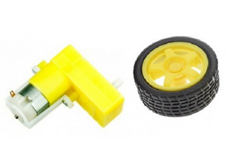
\includegraphics[scale=0.7]{figuras/kit_motor_reducao.png}
		\caption{Kit motor redução.}
		\label{img:kit_motor_reducao}
	\end{figure}

\begin{figure}[H]
	\centering
	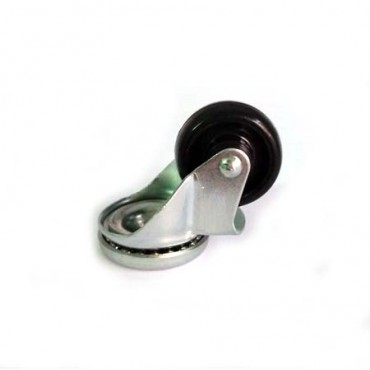
\includegraphics[scale=0.7]{figuras/roda_boba.png}
	\caption{Roda do tipo esfera com dimensão.}
	\label{img:roda_boba}
\end{figure}
	
	Na tabela abaixo estão apresentadas as especificações do motor utilizado.

	TABELA ERRADA, SEM INFORMAÇÕES.

	Verificar esta seção.. tudo bugado.

% section estrutura_do_robô (end)